\documentclass[twoside]{article}
% \documentclass[a4paper,10pt,twoside]{article}
\usepackage{afterpage}			% met landscape sans blanc
\usepackage[british]{babel}
\usepackage{caption}
\usepackage{color}			% Gestion de la couleur
\usepackage{fancyhdr}			% en-tête et pied-de-page
\usepackage{graphicx} 			% Insère image (eps, ps)
\usepackage{hyperref}			% Gère les liens hypertexte
\usepackage[utf8]{inputenc}
\usepackage{longtable}
\usepackage{lscape}			% Format landscape
\usepackage[round]{natbib}		% Bibliographie
\usepackage{pxfonts}
\usepackage[load-configurations = abbreviations]{siunitx}
\usepackage[skip=10pt]{subcaption}	% Figure composite
\usepackage{textcomp}
\usepackage{url}

\usepackage{geometry}
 \geometry{
 a4paper,
 total={210mm,297mm},
 left=20mm,
 right=20mm,
 top=30mm,
 bottom=30mm,
 }
 
 \newcommand\registred{\textsuperscript{\tiny\textregistered}}
 
%%%%%%%%%%%%%%%%%%%%%%%%%%%%%%%%%%%%%%%%%%%%%%%%%%%%%%%%%%%%%%%%%%%%
%% Folders
%%%%%%%%%%%%%%%%%%%%%%%%%%%%%%%%%%%%%%%%%%%%%%%%%%%%%%%%%%%%%%%%%%%%

\graphicspath{
	{figs/}
	{graphs/}
	}

%%%%%%%%%%%%%%%%%%%%%%%%%%%%%%%%%%%%%%%%%%%%%%%%%%%%%%%%%%%%%%%%%%%%
%% Links
%%%%%%%%%%%%%%%%%%%%%%%%%%%%%%%%%%%%%%%%%%%%%%%%%%%%%%%%%%%%%%%%%%%%

\definecolor{vert}{RGB}{32,121,35}
\definecolor{navy}{RGB}{0,95,190}
\urlstyle{sf} \hypersetup{
	unicode = true,
	colorlinks = true,
	urlcolor = {navy},
	linkcolor = {navy},
	citecolor = vert,
	pdfauthor = {Jérémy Ragusa, Lina Maria Ospina Ostios, Silvia Spezzaferri, Pascal Kindler},
	pdftitle = {Revision of the planktonic foraminiferal biostratigraphy of the Voirons Flysch (Chablais Prealps, Haute-Savoie, France)},
	pdfsubject = {},
	pdfkeywords = {biostratigraphy; flysch; Palaeogene; planktonic foraminifera; Valais domain; Voirons-Wägital complex},
	pdfcreator = {Jérémy Ragusa},
	pdfproducer = {LaTeX et pdflatex}
	}
	
%%%%%%%%%%%%%%%%%%%%%%%%%%%%%%%%%%%%%%%%%%%%%%%%%%%%%%%%%%%%%%%%%%%%
%% Headers and Footers
%%%%%%%%%%%%%%%%%%%%%%%%%%%%%%%%%%%%%%%%%%%%%%%%%%%%%%%%%%%%%%%%%%%%

\fancypagestyle{firststyle}{
   \fancyhf{}
   \fancyfoot{}
   \renewcommand{\headrulewidth}{0pt}
}

\fancypagestyle{plain}{
	\fancyhead[LO]{Swiss J Geosci}
	\fancyhead[RO]{DOI:10.1007/s00015-018-0314-7}
	\renewcommand{\headrulewidth}{0.4pt}
	}
	
\fancyhead[LO]{Swiss J Geosci (2018)}
\fancyhead[RO]{\thepage}
\fancyhead[RE]{Swiss J Geosci (2018)}
\fancyhead[LE]{\thepage}
\fancyfoot{}
\pagestyle{fancy}

%%%%%%%%%%%%%%%%%%%%%%%%%%%%%%%%%%%%%%%%%%%%%%%%%%%%%%%%%%%%%%%%%%%%
%% Units
%%%%%%%%%%%%%%%%%%%%%%%%%%%%%%%%%%%%%%%%%%%%%%%%%%%%%%%%%%%%%%%%%%%%

\sisetup{detect-all,
	 inter-unit-separator=$\cdot$,
	 range-phrase=--, % Utilise le tiret court pour dire "de... à"
	 range-units=single, % Cache l'unité sur la première borne
	}

\DeclareSIUnit{\Ma}{Ma}

%%%%%%%%%%%%%%%%%%%%%%%%%%%%%%%%%%%%%%%%%%%%%%%%%%%%%%%%%%%%%%%%%%%%
%% Bibliography
%%%%%%%%%%%%%%%%%%%%%%%%%%%%%%%%%%%%%%%%%%%%%%%%%%%%%%%%%%%%%%%%%%%%

\setlength{\bibsep}{0.1cm}		% Intervalle entre références
\bibpunct{(}{)}{ ;}{a}{,}{,} 		% Mise en forme références

%%%%%%%%%%%%%%%%%%%%%%%%%%%%%%%%%%%%%%%%%%%%%%%%%%%%%%%%%%%%%%%%%%%%
%% Title and author layout
%%%%%%%%%%%%%%%%%%%%%%%%%%%%%%%%%%%%%%%%%%%%%%%%%%%%%%%%%%%%%%%%%%%%

\makeatletter
\renewcommand{\maketitle}{\bgroup\setlength{\parindent}{0pt}
\begin{flushleft}
  \Large{\textbf{\@title}}
  \bigskip
  
  \small{\@author}
\end{flushleft}\egroup
}
\makeatother

%%%%%%%%%%%%%%%%%%%%%%%%%%%%%%%%%%%%%%%%%%%%%%%%%%%%%%%%%%%%%%%%%%%%

\title{Revision of the planktonic foraminiferal biostratigraphy of the Voirons Flysch (Chablais Prealps, Haute-Savoie, France)}
\author{\textbf{Jérémy Ragusa}\textsuperscript{1}, Lina Maria Ospina‐Ostios\textsuperscript{2}, Silvia Spezzaferri\textsuperscript{3}, Pascal Kindler\textsuperscript{1}}
\date{}

\begin{document}

\maketitle

\thispagestyle{firststyle}

\begin{flushleft}
{\smallskip{\footnotesize%
  \textsuperscript{1} University of Geneva, Department of Earth Sciences, 13, Rue des Maraîchers, CH-1205 Geneva, Switzerland\par  
  \textit{Contact}: J\'er\'emy~Ragusa (\texttt{\url{jeremy.ragusa@hotmail.fr}})\par
  \addvspace{\medskipamount}
  \textsuperscript{2} Universidad del Valle, Escuela de Ingeniería Civil y Geomática, Cali, Colombia\par
  \addvspace{\medskipamount}
  \textsuperscript{3} Unit of Earth Sciences, Department of Geosciences, University of Fribourg, Chemin du Musée 6, 1700 Fribourg, Switzerland\par
  \medskip
  \normalsize{Swiss Journal of Geosciences, x, doi: \href{https://doi.org/10.1007/s00015-018-0314-7}{10.1007/s00015-018-0314-7}}
  \medskip
}}
\end{flushleft}

\begin{abstract}
The ages obtained from planktonic foraminiferal assemblages retrieved from two exposures in the Gurnigel Flysch and from the re-examination of similar material gathered by previous researchers from the Voirons Flysch reveal only minor discrepancies with previous studies based on nannofossil biostratigraphy. In contrast, major divergences between this work and previous studies on the Voirons Flysch also based on planktonic foraminifera have been identified. They are generally related to distinct approaches in species classification and the use of different zonal schemes. Based on our data, the age of the Voirons Flysch extends from the Early Eocene (planktonic foraminiferal zone P7) to the Middle Eocene (planktonic foraminiferal zone P12). Contrasting with claims made in earlier studies, no specimen of Late Eocene or Early Oligocene age has been observed in the revised material. However, we cannot exclude a younger age (possibly Late Eocene) for the upper portion of this flysch from which we did not revise any sample. Thus, more research and sampling are needed to resolve this question. The palaeogeographic origin of the Voirons-Wägital complex as well as the sedimentation history of these flyschs need now to be re-evaluated in light of this revised biostratigraphic data.
\end{abstract}

\begin{center}
{\small{\bf Keywords}\par
\smallskip
biostratigraphy; flysch; Palaeogene; planktonic foraminifera; Valais domain; Voirons-Wägital complex\par}
\end{center}

\section{Introduction}

The term “flysch” (e.g. \citealp{Studer1848,Wildi1987,Homewood1988}) designates terrigenous sediments of Alpine basins that have been redeposited in the deep sea by gravity-flow processes during a period of convergence. Flysch deposits primarily consist of alternations of shales, sandstones and conglomerates showing evidence of mass-flow transport (i.e. turbidites s.l., \citep{Mutti2009}). They represent the last depositional stage in successive palaeogeographic domains before their subduction and subsequent accretion into a sedimentary accretionary prism \citep{Kuenen1953,Homewood1988,Stampfli2002b}). Constraining the age of flysch units is thus critical for reconstructing the kinematics of orogenies \citep{Stampfli2002b,Stampfli2009,Handy2010}.\par
Micro- and nannofossils are the most powerful tools for dating marine detrital sequences. This task is however greatly complicated due to the importance of reworking processes on the sea floor, which may incorporate material derived from older sediments in the flysch (e.g. \citealp{Morel1980b,Mulder2001}). The most appropriate dating technique consists in retrieving micro- and nannofossils from the pelagic beds interspersed in flysch successions (e.g. \citealp{Ujetz1996}). Unfortunately, the preservation of hemipelagic layers is variable, and depends on the depositional environment. These layers are absent or rare in the amalgamated coarse-grained sandstones to conglomerates of channel settings, and can be confused with the fine-grained division of Bouma sequences (Te; \citealp{Bouma1962}) in lobe settings \citep{Mutti2003} commonly forming the bulk of flysch shales.\par
Initial attempts to date flysch deposits were based on larger benthic foraminifera \citep{Pilloud1936,Lombard1940a,Schaub1951,Rigassi1958,Cogulu1961,Schaub1965}. However, these organisms are mostly reworked from neighbouring carbonate platforms where they thrived during the Palaeogene \citep{Scheibner2008a}. Calcareous nannofossils provided the first accurate biostratigraphic determinations in Alpine flyschs \citep{Hekel1968,JanduChene1975c,Stuijvenberg1980a}. More recently, planktonic foraminifera biostratigraphy was also applied in the Voirons Flysch \citep{Ujetz1996,Frebourg2006,Ospina-Ostios2013,Ospina-Ostios2017}.\par

\afterpage{
	\begin{figure}[htp!]
		\centering
		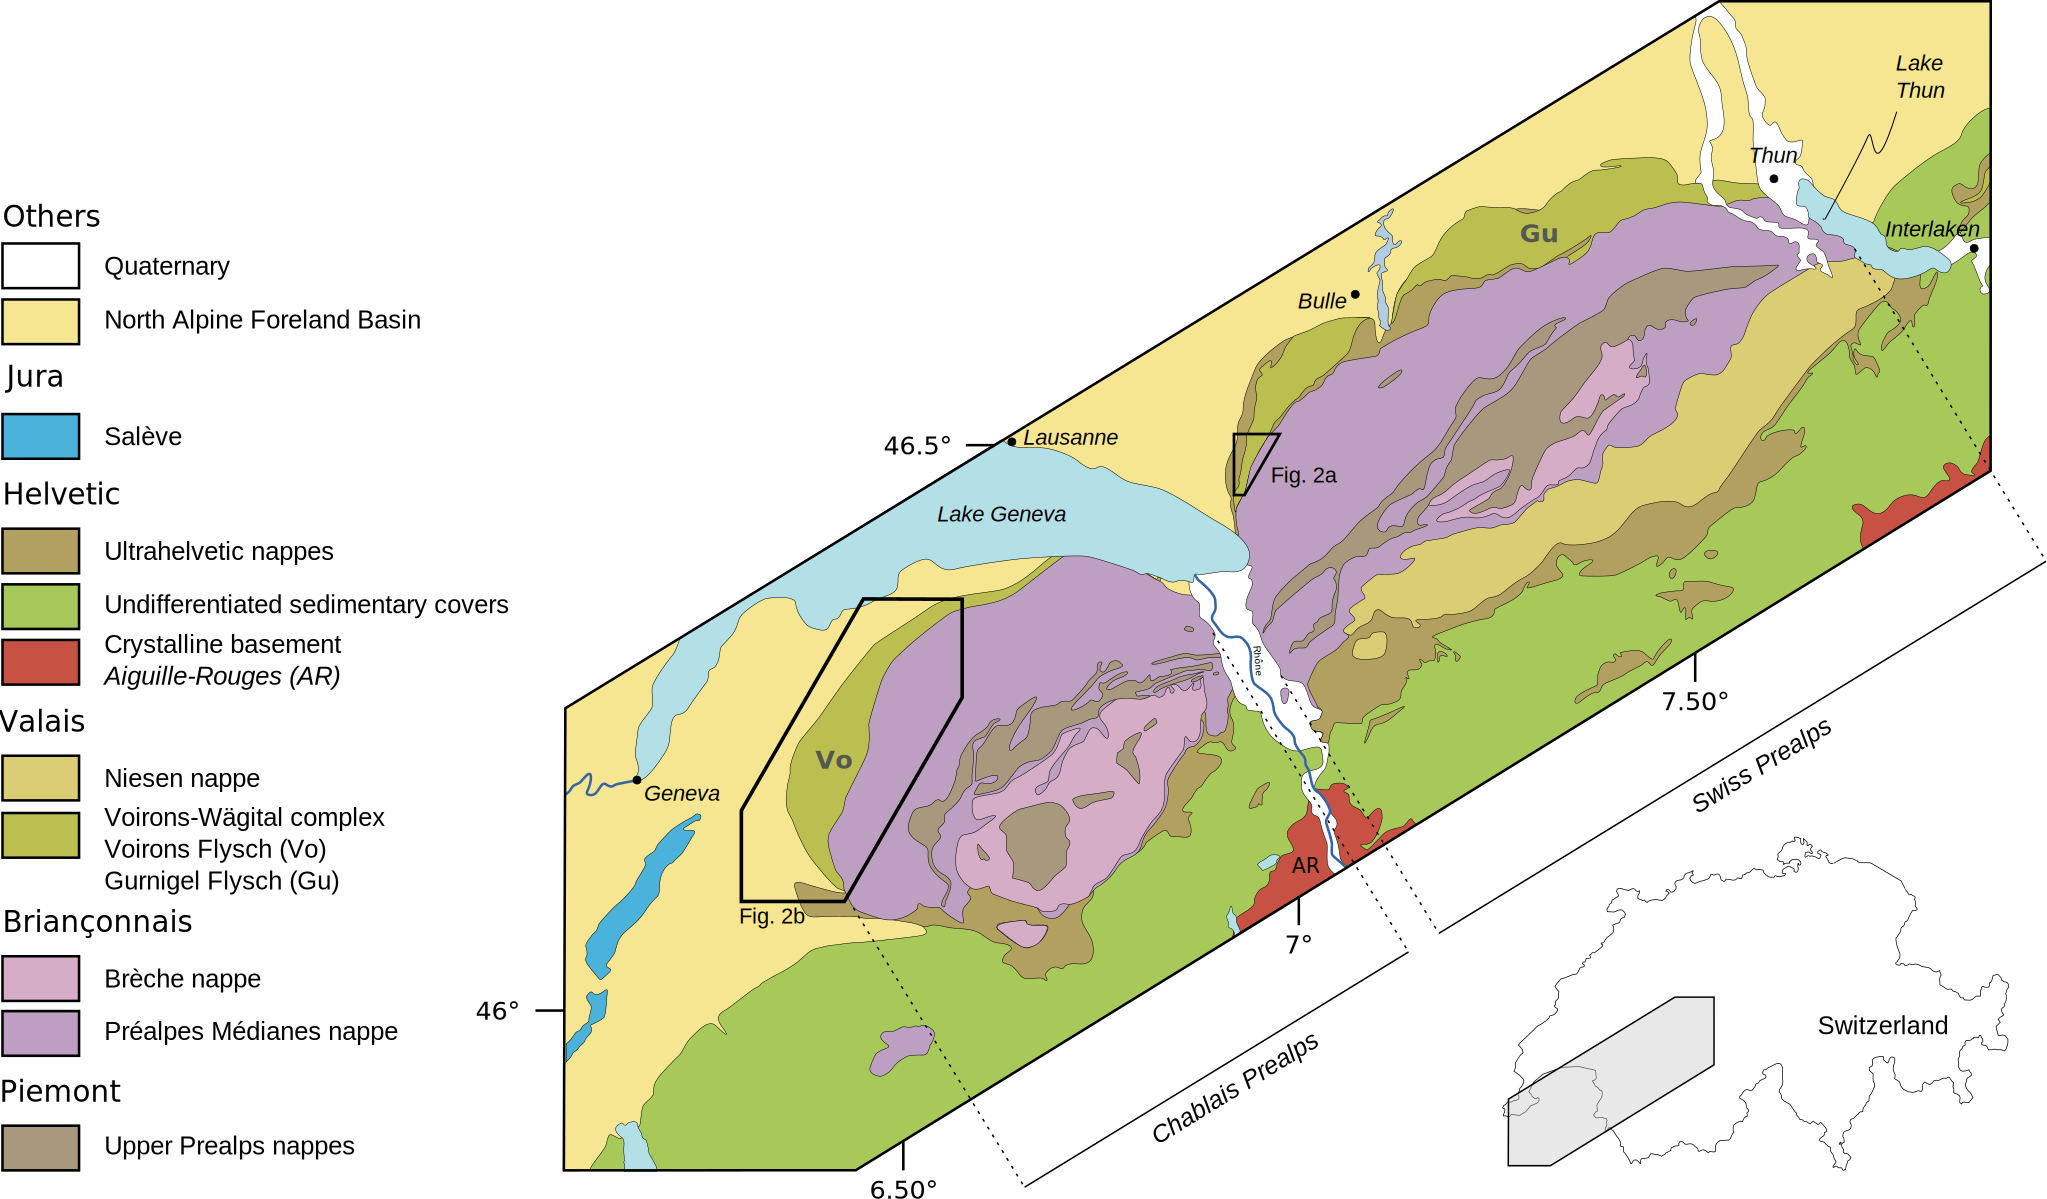
\includegraphics[width=\textwidth]{Fig1.pdf}
		\caption{test.}
		\label{fig:Fig1}
	\end{figure}
	}

The flyschs exposed in the Chablais and Swiss Prealps (Fig. 1) range in age from the Late Cretaceous to the Oligocene \citep{Matter1980,Homewood1982,Caron1989}. As illustrated in \cite{Caron1989}, the oldest flysch units are derived from the most internal palaeogeographic realms (e.g. the South-Penninic domain), and form the upper portion of the Prealpine nappes stack (e.g. the Gets nappe). By contrast, the youngest ones, known as the North Helvetic Flysch group \citep{Menkveld-Gfeller2016}, originate from more external domains (e.g. the inner portion of the North Alpine foreland basin), and occur at the base of the nappe sequence. Determining the palaeogeographic origin of flyschs is fairly easy when such a succession occurs in stratigraphic continuity with pre-flysch deposits, as in the Briançonnais domain (Médianes Flysch, \citealp{Caron1980}; Brèche Flysch, \citealp{DallAgnolo2000}). However, in the Chablais and Swiss Prealps, several flysch slices and nappes are indeed isolated from their substrate and, consequently, their palaeogeographic attribution largely depends on their inferred age.\par
This is the case of the Voirons Flysch, which forms the westernmost part of the former Gurnigel nappe, now called the Voirons-Wägital complex. This complex has long been considered as related to the Ultrahelvetic domain due to its low structural position \citep{Lombard1940a,Trumpy1960,Hsu1971}. In the late 20th century, it was attributed to the South-Penninic domain based on micropalaeontological data and because of its petrographic resemblance with the Sarine nappe (Upper Prealps; \citealp{Caron1976,Caron1980,Stuijvenberg1980b,Caron1989,Gasinski1997}. In the past two decades, several researchers \citep{Ujetz1996,Coppo1999,Frebourg2006,Ospina-Ostios2013,Ospina-Ostios2017} found planktonic foraminiferal assemblages indicating a Middle Eocene to Early Oligocene age in the Voirons Flysch, which precludes a South-Penninic origin for this unit. Consequently, and corroborating the ideas of \cite{Schmid2005} as well as the conclusions of \cite{Trumpy2006} for the easternmost part of the Voirons-Wägital complex (e.g. the Iberg Klippes), the Voirons Flysch was attributed to the Valais realm (Ospina-Ostios et al., 2013, Ragusa et al., 2017), which appears to agree better with its present-day low structural position but this is not the subject of the present paper.\par
The primary goal of this study was to apply planktonic foraminiferal biostratigraphy to exposures of the Voirons-Wägital complex in the western part of Switzerland to possibly confirm and substantiate the research made in the Voirons massif \citep{Ujetz1996,Coppo1999,Frebourg2006,Ospina-Ostios2013,Ospina-Ostios2017}. However, our initial results from two outcrops in that area convinced us about the need of a thorough revision of the data from the Voirons Flysch, which is now the main aim of this paper.\par

\section{Geological Setting}

The Voirons-Wägital complex, which includes the Voirons, the Gurnigel, the Schlieren and the Wägital Flyschs (Fig. 1), forms moderate-elevation, commonly forest-covered mountains (e.g. the Voirons, the Niremont) on the external edge of the Chablais and Swiss Prealps. This complex occurs near the base of the Prealpine nappe stack, between a complex zone comprising tectonic mélanges and Ultrahelvetic slices below and the Préalpes Médianes nappe above (Figs. 1 and 2), and consists of vertically stacked flysch successions generally forming a large synform with numerous internal folds \citep{Weidmann1976a,Morel1980b,Winkler1983,Ospina-Ostios2017}. In this paper, we are only concerned with the Gurnigel and the Voirons Flyschs (Figs. 2a and 2b, respectively). The former encompasses a succession of five units (Flyschs 1 to 5; Fig. 3a), discriminated by subtle differences in lithology, that have been dated from the Maastrichtian to the Middle Eocene by calcareous nannofossil biostratigraphy (Figs. 3a and 4; \citealp{Weidmann1976a,Morel1980b}). The latter includes four formations (from base to top, Fig. 3b): the Voirons Sandstone, the Vouan Conglomerate, the Boëge Marl, and the Bruant Sandstone formations \citep{Ragusa2015}. Originally attributed to a time interval from the Danian to the Priabonian (nannofossil zones NP2 to NP18; Fig. 5) based on coccolith and dinoflagellate assemblages \citep{JanduChene1975c,Stuijvenberg1980a,Stuijvenberg1980b}, this flysch succession has more recently been dated to the Middle Eocene - Early Oligocene (Figs. 3b and 5; planktonic foraminiferal zones P13 to P20) based on planktonic foraminifera \citep{Ujetz1996,Coppo1999,Frebourg2006,Ospina-Ostios2013,Ospina-Ostios2017}. No nannofossils younger than the Priabonian has ever been found in these lithologies.\par

\afterpage{
	\begin{figure}[htp!]
		\centering
		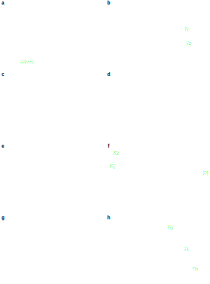
\includegraphics[width=\textwidth]{Fig2.pdf}
		\caption{test.}
		\label{fig:Fig2}
	\end{figure}
	}

The selected outcrops are found in the southern part of the Gurnigel  Flysch (Figs. 1 and 2). Located to the SE of Châtel-St-Denis, in the Veveyse de Fégire gorges, the first section exposes the lower to middle Eocene Flysch 3 (Fig. 3a; \citealp{Weidmann1976a}). The second outcrop is in the Veveyse de Châtel valley, to the N of Les Paccots, and comprises lithologies attributed to the middle Eocene Flysch 4 (Fig. 3a; \citealp{Morel1980b}). The revised samples from the Voirons massif have been borrowed from the collections of Lina Ospina-Ostios and Grégory Frébourg (samples LMO and GF, respectively), both of which are deposited at the Department of Earth Sciences of the University of Geneva. These samples represent all stratigraphic units from the Voirons Flysch, except for the Bruant Sandstone Fm. (Fig. 2). GPS coordinates and stratigraphic attribution of these samples are given in Table 1.\par
The Schlieren Flysch \citep{Winkler1983,Winkler1984} comprises a lithostratigraphic succession similar to that of the Gurnigel Flysch. Nannofossil biostratigraphy gave a Late Maastrichtian to late Ypresian age to this flysch (Late Maastrichtian to nannofossil zone NP14; \citealp{Winkler1984,Caron1989}; Fig. 6). The Wägital Flysch \citep{Winkler1985a} is roughly subdivided into three units, and extends from the Campanian to the Middle Eocene (Fig. 6).

\afterpage{
	\begin{figure}[htp!]
		\centering
		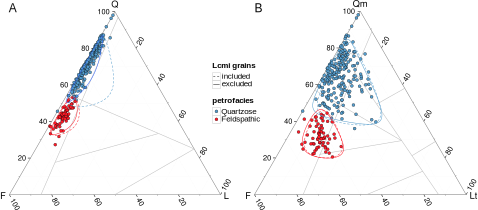
\includegraphics[angle=270,width=\textwidth]{Fig3.pdf}
		\caption{test.}
		\label{fig:Fig3}
	\end{figure}
	}

\section{Methods}

In turbidites, the upper portions of thick shale beds have the highest probability to represent pelagic deposits \citep{Mutti2003,Mulder2001}. We thus looked for such layers in the selected exposures from the Gurnigel  Flysch, and gathered ca. 500 g of material at depth with a clean spatula to avoid field contamination. Samples were then disaggregated with gasoline, washed, and wet-sieved through 90–1000 µm sieves for qualitative planktonic foraminiferal analyses. For the Voirons Flysch, we simply used the leftover residues of samples collected by previous researchers \citep{Frebourg2006,Ospina-Ostios2017}. After manual picking, selected specimens were photographed with a Nikon digital camera mounted on a Nikon SMZ18 stereomicroscope fitted with a 0.5x SHR Plan Apo objective. Images were taken of each specimen using the NIS Elements Imaging Software v4.60. Finally, the foraminifera illustrated in the plates published by \cite{Ospina-Ostios2013} and \cite{Ospina-Ostios2017} were re-examined and, in some cases, re-determined. Species determinations and age ranges are based on \cite{Pearson2006} and \cite{Wade2011a}. The P Zones of \cite{Berggren1995a} are also used in the text to facilitate comparison with previous works. The comparison with E and P Zones are reported in Figs. 4, 5 and 6. Nannofossil biostratigraphy is based on \cite{Martini1971} (Fig. 6).\par
	
\section{Results}

\subsection{Gurnigel Flysch}

The exposure in the Veveyse de Fégire gorges (Figs. 2 and 7a; GPS coordinates in Table 1) consists of well-exposed, shale-dominated, distal turbidites (F8 - F9; \citealp{Mutti2003}) characterized by the Tb-Te intervals of the Bouma sequence. The thickness of sandstone beds seldom exceeds 10 cm, whereas that of intercalated shales varies between 50 cm and 1 m. Strata occur in normal position, and dip sharply (60°) towards the East. These turbidites were originally correlated with the Early to Middle Eocene (nannofossil zones NP 12 to NP 15; \citealp{Weidmann1976a}). Samples JR 377 and JR 378 (Fig. 3a) were collected from pelagic marls identified by their greenish colour that contrasts with the dark-grey tint of the Te intervals (Fig. 7b). The assemblage of poorly preserved planktonic foraminifera retrieved from these samples contains acarinids (Online Resource 1), and suggests also an Early to Middle Eocene age (planktonic foraminiferal zones E7b or P9) for this exposure.\par

\afterpage{
	\begin{figure}[htp!]
		\centering
		\includegraphics[angle=270,width=\textwidth]{Fig4.pdf}
		\caption{test.}
		\label{fig:Fig4}
	\end{figure}
	}

The Veveyse de Châtel outcrop (Figs. 2 and 7c; GPS coordinates in Table 1) likewise shows distal turbidites (F8 - F9; \citealp{Mutti2003}) with dm-scale, bioturbated, shaly intervals and thin (5 to 20 cm) laminated sandstone beds (Tb-Td). This succession is in normal position and displays a low dip (30°) towards the SE (Fig. 7c). A few pebbly sandstone beds (F2; \citealp{Mutti2003}) occur near the top of the exposure. These deposits were previously attributed to the Middle Eocene (nannofossil zones NP 15 to NP 16; \citealp{Weidmann1976a,Morel1980b}). Sample NPK 317 was collected from grey marls located just below a 5 cm-thick sandstone bed (Fig. 7d). The assemblage of poorly preserved planktonic foraminifera found in this sample (Online Resource 1 and 2) gave an age ranging from the late Early Eocene to the late Middle Eocene (planktonic foraminiferal zones E7b to E11, or P9 to P12).\par

\subsection{Voirons Flysch}

The residues of five samples regularly distributed within the sandstone-dominated Voirons Sandstone Fm. were re-picked and re-examined. Their geographic and stratigraphic positions are given in Figures 2, 3b and Table 1. Previous studies based on nannofossils \citep{JanduChene1975c,Stuijvenberg1980a} and planktonic foraminifera \citep{Ospina-Ostios2013,Ospina-Ostios2017} placed this formation in the Paleocene to Middle Eocene (nannofossil zones NP2 to NP16) and in the Middle Eocene to Early Oligocene (planktonic foraminiferal zones P13 to P19), respectively. The planktonic foraminiferal assemblages, some of them well-preserved (e.g. sample LMO042), are presented in Table 2. Collectively, these revised data constrain the age of the Voirons Sandstone Fm. between the Early and the Middle Eocene (planktonic foraminiferal zones E5 to E9, or P7 to P11). Reworked specimens of Cretaceous and Paleocene age have also been observed in these assemblages.
Likewise, the residues of four samples gathered from rare shaly intervals or mud pebbles (e.g. sample GF 269) scattered in the coarse-grained Vouan Conglomerate Fm. were reconsidered. The geographic and stratigraphic position of the outcrops from which they were collected are given in Figures 2, 3b and Table 1, respectively. Previous studies based on nannofossils \citep{JanduChene1975c,Stuijvenberg1980a} and planktonic foraminifera \citep{Frebourg2006,Ospina-Ostios2013,Ospina-Ostios2017} placed this formation in the Middle Eocene (nannofossil zones NP 15 to NP16) and in the late Middle Eocene to Early Oligocene (planktonic foraminiferal zones P15 to P19), respectively. The planktonic foraminiferal assemblages are shown in Online Resource 1, and selected specimens are illustrated in Online Resource 2 and 3. The assemblages from all four samples contain numerous reworked forms, and yield up to three ages in the Eocene. Sample LMO056 gave the most recent and precise age in the Middle Eocene (planktonic foraminiferal zone E11 or P12), which overlaps the Lutetian - Bartonian boundary.\par
Only two samples from the lower part of the shale-dominated Boëge Marl Fm. were re-evaluated. Section from upper layers are barren of planktonic specimens (Dranse outcrop; \citealp{JanduChene1975c}). Their geographic and stratigraphic positions are  in Figures 2, 3b and Table 1. The planktonic foraminiferal assemblages are listed in Online Resource 1, and selected specimens are illustrated in Online Resource 2 and 3. Previous studies based on nannofossils \citep{Stuijvenberg1980a} and planktonic foraminifera \citep{Coppo1999,Ospina-Ostios2013,Ospina-Ostios2017} placed this formation in the Late Eocene (nannofossil zones NP18) and in the late Middle Eocene to Early Oligocene (planktonic foraminiferal zones P13 to P20), respectively. Like the material retrieved from the Vouan Conglomerate Fm., the planktonic foraminiferal assemblages identified in these two samples contain numerous reworked Early to Middle Eocene and even Cretaceous forms (e.g. hedbergellids in LMO292). The youngest age obtained for both samples is Middle Eocene (planktonic foraminiferal zones E11 or P12). It is identical to that obtained from the underlying Vouan Conglomerate Fm. Due to the paucity of shaly layers, no samples were collected from the sandstone-dominated, highly tectonised Bruant Sandstone Fm.\par
Thus, according to our new and revised data, the age of the Voirons fFlysch ranges from the Early Eocene to the late Middle Eocene, i.e. from the Late Ypresian to the Early Bartonian (planktonic foraminiferal zones P7 to P12). No specimen of planktonic foraminifera with a range restricted to the Late Eocene or Early Oligocene age was detected in the studied residues.\par

% \afterpage{
	\begin{figure}[htp!]
		\centering
		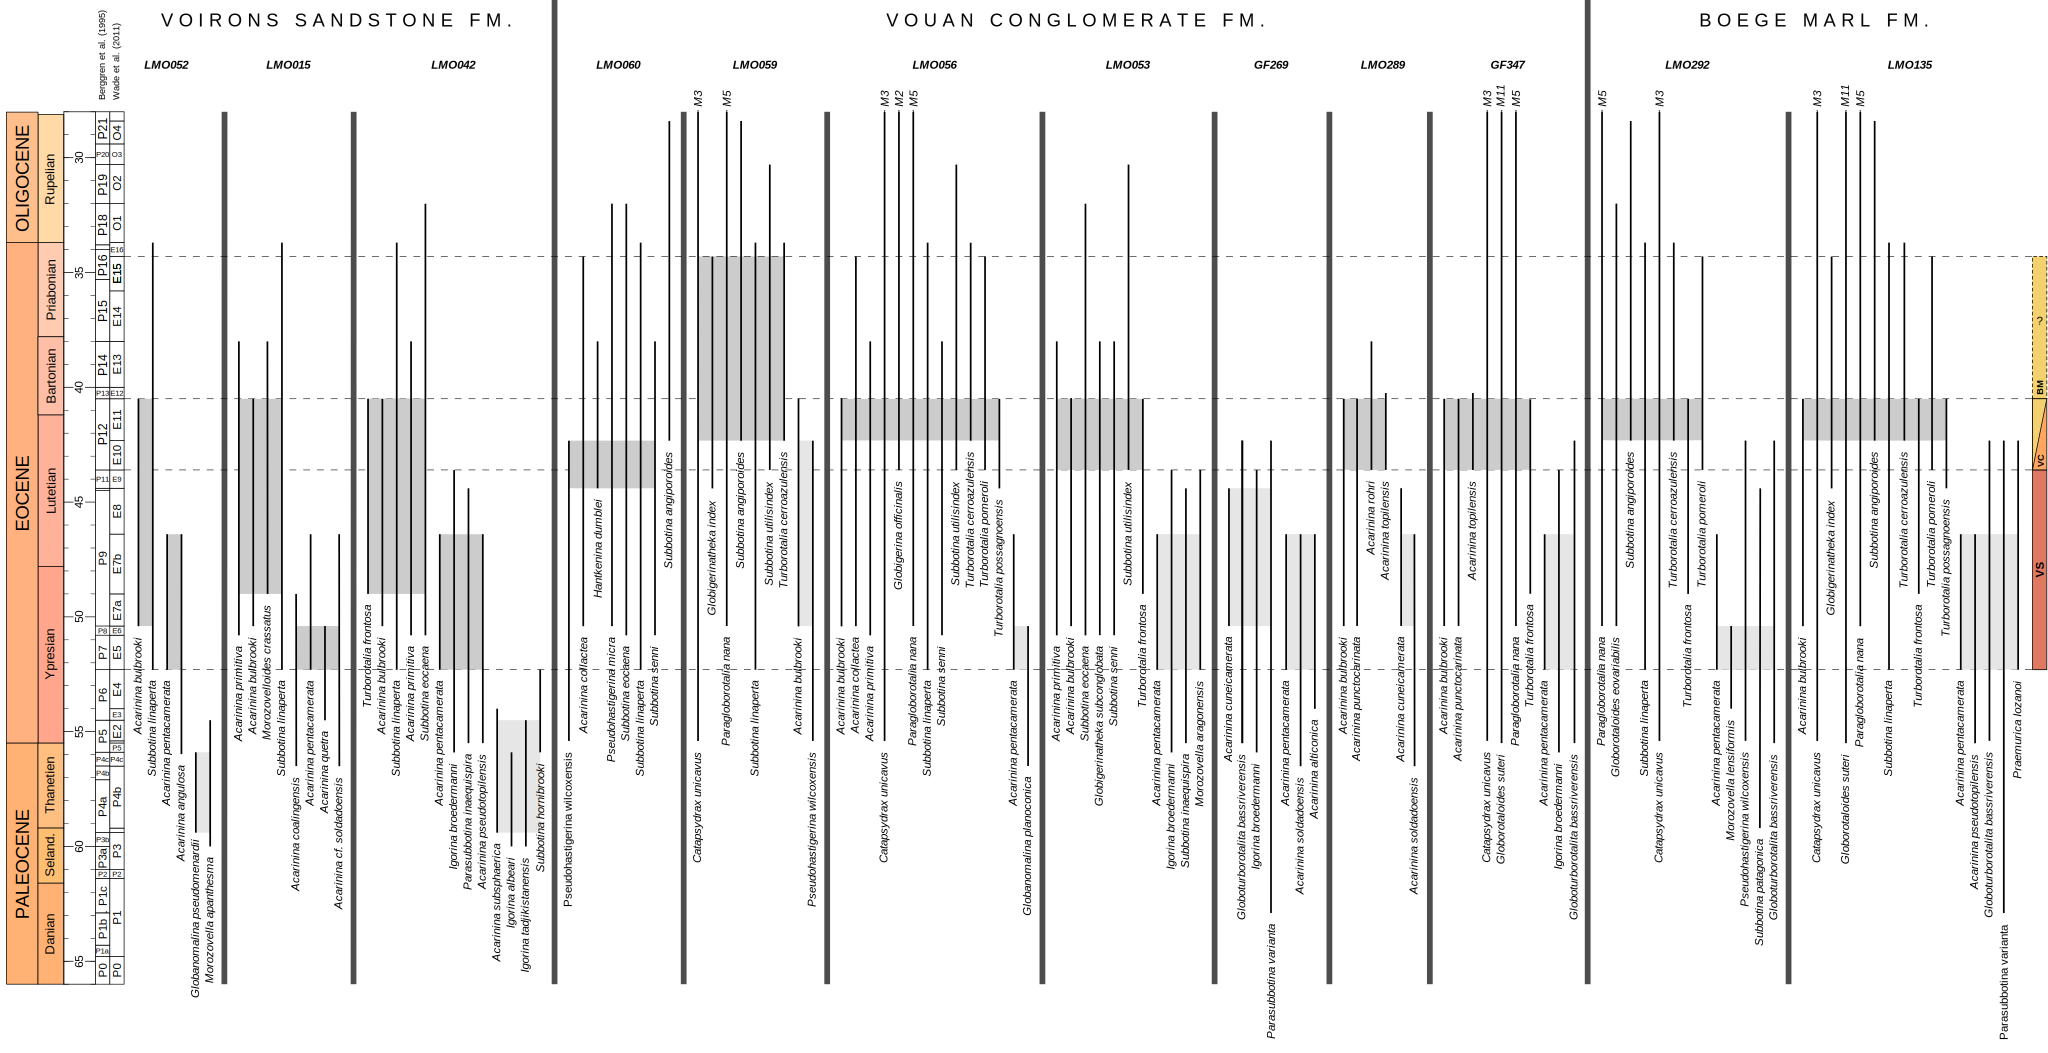
\includegraphics[angle=270,width=0.75\textwidth]{Fig5.pdf}
		\caption{test.}
		\label{fig:Fig5}
	\end{figure}
% 	}

\section{Discussion}

\subsection{Comparison with previous biostratigraphic results}

The foraminiferal ages acquired from the two samples collected from the Gurnigel Flysch agree with the previous biostratigraphic data based on nannofossils \citep{Weidmann1976a,Morel1980b}. By contrast, our new data do not fully agree with any biostratigraphic result previously found in the Voirons Flysch. The older ages obtained from nannofossil analyses \citep{JanduChene1975c,Stuijvenberg1980b} for the onset of flysch sedimentation (Danian or Thanetian versus Ypresian) can be explained by considering that the Paleocene forms observed by these authors have been reworked (see Section 5.2). Similarly, the slight offset between the nannofossil age (Early Priabonian; \citealp{Stuijvenberg1980b}) and our data (Early Bartonian) for the end of flysch deposition could likely be related to the small number of revisited samples from the Boëge Marl Fm. However, the important discrepancies between our study and those of \citep{Ospina-Ostios2013} and \citep{Ospina-Ostios2017}, all of which relying on planktonic foraminifera biostratigraphy, cannot be easily dismissed, and are further discussed below.\par

\subsection{Discrepancies in planktonic foraminifera biostratigraphy}

The expansion of the Ocean Drilling Program (ODP) in the 80’s and more recently of the Integrated Ocean Drilling and International Discovery Programs (IODP) have added a huge amount of information about planktonic foraminiferal ranges and taxonomy with the recovery of continuous sedimentary sequences and very well-preserved planktonic foraminiferal species. The pioneering comprehensive work of \cite{Toumarkine1985} on Palaeogene planktonic foraminifera has been revised and completed in the Atlases of Paleocene and Eocene Planktonic Foraminifera compiled by the Palaeogene Planktonic Foraminifera Working Groups (PPFGW) active since 1987 \citep{Olsson1999,Pearson2006}. These comprehensive monographies not only present a new biologically guided classification of planktonic foraminifera based on the characteristics of the wall textures, but also refined ranges for each species at a global scale. The advantage of these atlases is that holotypes and, in some cases, also paratypes of each species are imaged, mostly with the environmental SEM, and we have now the documentation of type specimens that, in most cases, were only illustrated by drawings.\par
\cite{Ospina-Ostios2013} and \cite{Ospina-Ostios2017} mostly used the taxonomy and species ranges reported in \cite{Toumarkine1985} and the time scale of \citep{Luterbacher2004}. The more recent biostratigraphy and taxonomic works of \cite{Pearson2006} and \cite{Wade2011a} have been only used to update generic names. Additionally, they have not used the classification of planktonic foraminifera based on wall texture. Although the planktonic foraminifera from the Gurnigel Flysch are very poorly preserved, it is still possible to identify the details of the wall texture for most specimens. One example is the specimen illustrated on Online Resource 3 (6b) of \cite{Ospina-Ostios2013} identified as Tenuitellinata angustiumbilicata. This form shows a coarsely cancellate wall texture typical of macroperforate genera (e.g. Paragloborotalia or Subbotina) instead of the microperforate wall texture typical of the genus Tenuitellinata. The main discrepancies between the studies of \cite{Ospina-Ostios2013} and \cite{Ospina-Ostios2017} and the present work are generally due to the different approaches in classification of species and the use of different zonal schemes.\par
Thus, based on our revision of previous data, the onset of sedimentation of the Voirons Flysch spans the interval zones P7-P9 (as in \citealp{Berggren1995a}) corresponding to Zones E5-E7 of \cite{Wade2011a}, whereas the end of deposition can be mostly restricted to Zone P12 (as in \citealp{Berggren1995a}) corresponding to Zones E10-E11 \citep{Wade2011a}. However, we cannot rule out that sedimentation continued as late as the Priabonian (Figs. 5 and 6) because we only revised two samples from the lower part of the Boëge Marl Fm. and none from the overlying Bruant Sandstone Fm. Such an attribution would agree with previously obtained results based on nannofossil biostratigraphy that suggested an early Priabonian maximum age (nannofossil zone NP 18) for the Boëge Marl Fm. \citep{JanduChene1975c,Stuijvenberg1980b}).\par

\subsubsection{Reworking in the Voirons Flysch}

The comparison of biostratigraphic ranges allows to reconstruct some sedimentary processes throughout the Voirons Flysch. Samples of the Voirons Sandstone Fm. include reworked specimens of Late Paleocene age (Fig. 5). Such an age is not reported in the Voirons Flysch, and may be derived either from (1) extrabasinal marly successions or (2) an older upstream equivalent of the Voirons Sandstone Fm. The latter hypothesis suggests that, in contrast to the other flyschs from the Voirons-Wägital complex (Fig. 6), Paleocene sediments might have been tectonically removed during an early phase of thrusting. Similarly, the presence of Upper Cretaceous specimens (Campanian to Maastrichtian) may involve a contribution from basinal marls of Mesozoic age.\par
The Vouan Conglomerate Fm. consistently comprises specimens reworked from the Voirons Sandstone Fm. However, these elements are missing in the sample LMO060 collected from the lower part of this unit, indicating that reworking processes started after a short delay. This break can also be observed in the field where the basal part of the Vouan Conglomerate Fm. corresponds to a sandstone-marl alternation (Saxel upper quarry; \citealp{Ragusa2015}). In addition, the restricted range of sample GF269 (Fig. 5) suggests that the mud pebbles occurring within some beds of the Vouan Conglomerate Fm. may directly derive from the Voirons Sandstone Fm.\par
The biostratigraphic range of the Boëge Marl Fm. does not differ from that of the Vouan Conglomerate Fm. (Fig. 5), and also comprises reworked specimens from the Voirons Sandstone Fm. We suppose that the youngest age obtained from the Boëge Marl Fm. reflects reworking from the Vouan Conglomerate Fm. This marly succession corresponds to a starvation period, enabling the destabilisation of the turbiditic system. Hence, the obtained Lutetian – early Bartonian age may emphasize the remobilisation of upstream components of the Vouan Conglomerate Fm. basinward, corroborating the occurrence of one single conglomeratic bed at the base of the Boëge Marl Fm. \citep{Ragusa2015,Ospina-Ostios2017}. The presence of late Ypresian to Lutetian foraminifera also confirms a contribution from the Voirons Sandstone Fm. Finally, the occurrence of Upper Cretaceous specimens, that are missing in the Vouan Conglomerate Fm., also suggests that this unit originates from the same source as the Voirons Sandstone Fm., as previously confirmed by the similar detrital composition \citep{Ragusa2017a}. Consequently, sampling in the upper part of the unit, where detrital sedimentation rate increases, may better constrain the depositional age of the Boëge Marl Fm. which probably ends during Priabonian (planktonic foraminiferal zones E15 to P16) from calcareous nannofossil biostratigraphy.\par

\subsection{Comparison with the other flyschs of the Voirons-Wägital complex and palaeogeographic implications}

As the age of the Voirons Flysch is now constrained between the Ypresian and the Priabonian, the whole Voirons-Wägital complex ranges from the Campanian to the Late Eocene (Fig. 6), which corresponds to a ca. 49.7 Ma-long interval. The accumulation time of the Voirons Flysch (ca. 18 Ma) is shorter than that of the Gurnigel (ca. 26.6 Ma; \citealp{Weidmann1976a,Morel1980b}) and Schlieren Flyschs (ca. 19.7 Ma; \citealp{Winkler1983,Winkler1984}), whereas sedimentation of the Wägital Flysch lasted for about 45.6 Ma \citep{Winkler1985a}, spanning the time interval of the complex. The age ranges of the different flyschs become younger towards the West, suggesting a scissor-like closure of the basin \citep{Winkler1984}. Sedimentation started during the Late Cretaceous in the eastern units, but only initiated during the Early Eocene in the Voirons Flysch. Similarly, sedimentation ended in the Early Eocene in the Wägital Flysch, and probably stopped in the Late Eocene in the Voirons Flysch.\par

% \afterpage{
	\begin{figure}[htp!]
		\centering
		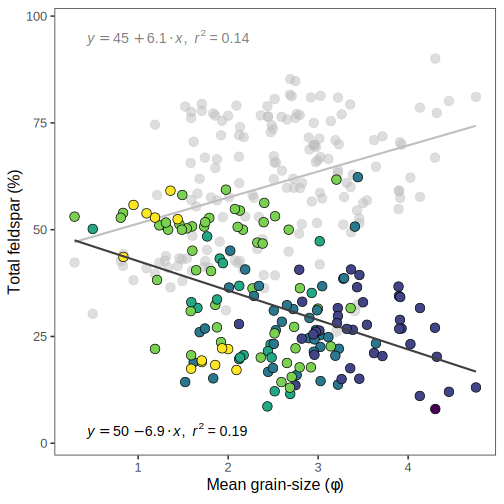
\includegraphics[width=\textwidth]{Fig6.pdf}
		\caption{test.}
		\label{fig:Fig6}
	\end{figure}
% 	}

Although our revised age of the Voirons Flysch is similar to that previously obtained from nannofossil biostratigraphy (Fig.6; \citealp{JanduChene1975c,Stuijvenberg1980b}), it does not necessarily re-establish a South Penninic origin for this unit, and for that matter for the whole Voirons-Wägital complex. These flyschs needed accommodation space before, during and after the deposition of the Briançonnais flyschs, especially of the Médiane Flysch (Fig. 6), which substantiates a palaeogeographic location in the Valais domain. Thus, our revised biostratigraphic data on the Voirons Flysch requires an update of the palaeogeographic model proposed by \cite{Ragusa2017a}, which will be detailed in a publication currently in preparation.\par

\afterpage{
	\begin{figure}[htp!]
		\centering
		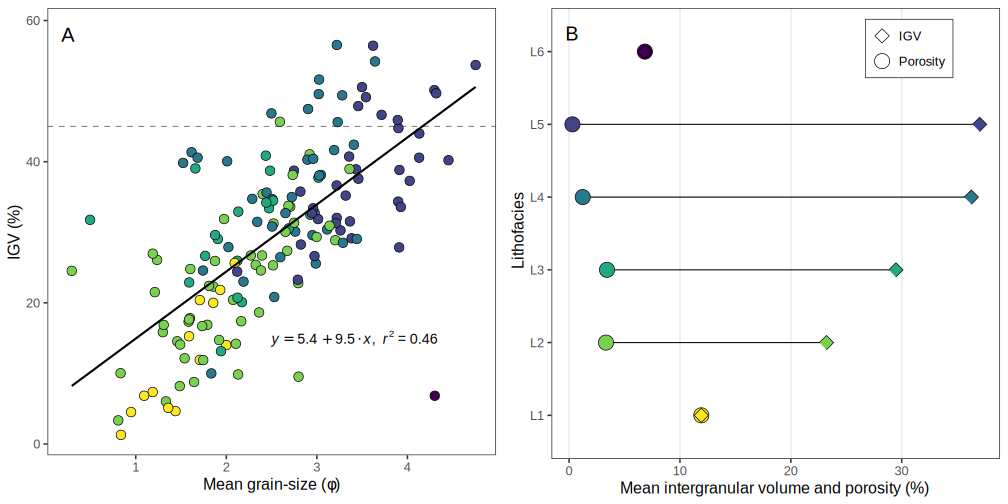
\includegraphics[width=\textwidth]{Fig7.jpg}
		\caption{test.}
		\label{fig:Fig7}
	\end{figure}
	}

\section{Conclusion}

The ages derived from the examination of planktonic foraminiferal assemblages from the Gurnigel Flysch and from our revision of material gathered by previous researchers from the Voirons Flysch reveal only minor discrepancies with earlier studies based on nannofossil biostratigraphy \citep{JanduChene1975c,Weidmann1976a,Morel1980b,Stuijvenberg1980a,Stuijvenberg1980b}. By contrast, there are major divergences between the results of our work and those of previous studies on the Voirons Flysch similarly based on planktonic foraminifera \citep{Ujetz1996,Coppo1999,Frebourg2006,Ospina-Ostios2013,Ospina-Ostios2017}. These discrepancies are generally related to the different approaches in species classification and the use of different zonal schemes. Based on our revised data, the age of the Voirons Flysch extends from the Early Eocene (planktonic foraminiferal zone E5 or P7) to the Middle Eocene (planktonic foraminiferal zone E11 or P12). Contrary to claims made in the aforementioned studies, specimens restricted to Late Eocene or Early Oligocene age have not been observed in the samples and in the illustrations we re-examined. However, we cannot exclude a younger age (possibly early Late Eocene) for the upper reaches of this flysch from which we did not have samples to re-examine. Further sampling in the upper part of the Boëge Marl Fm. and Bruant Sandstone Fm. will be investigate to better constrain the age from the top of the flysch deposition. Thus, additional research and sampling are needed to resolve this question. Finally, the palaeogeographic origin of the Voirons-Wägital complex as well as the sedimentation history of these flyschs need now to be re-evaluated in light of this revised biostratigraphic data.

\section*{Acknowledgements}

We are grateful to the constructive review and remarks of the Chief Editor and critical reviews by Ursula Menkveld.\par

\section*{Electronic supplementary materials}

The online version of this article contains supplementary material:
\begin{itemize}
 \item \emph{Supplementary material 1}: Framework composition of the Voirons Flysch following the Gazzi-Dickinson method
 \item \emph{Supplementary material 2}: SEM-EDS garnet geochemistry from the Voirons Flysch. Data include element and calculated oxide composition and enb-member abundance
 \item \emph{Supplementary material 3}: SEM-EDS tourmaline geochemistry from the Voirons Flysch. Data include element and calculated oxide composition
\end{itemize}

\bibliographystyle{apalike-doi}
\bibliography{Ragusa2018a}

\end{document}
